\documentclass[a4paper,12pt]{article}

\usepackage[14pt]{extsizes}
\usepackage{cmap}							% поиск в PDF
\usepackage{mathtext} 					% русские буквы в формулах
\usepackage[T2A]{fontenc}				% кодировка
\usepackage[utf8]{inputenc}				% кодировка исходного текста
\usepackage[english,russian]{babel}	% локализация и переносы
\usepackage{graphicx}
\usepackage{geometry}
\usepackage{amsmath}
\usepackage[table]{xcolor}
\setlength\extrarowheight{2pt}


\geometry{verbose, a4paper, tmargin=2cm, bmargin=2cm, lmargin=3cm, rmargin=2cm}
\author{Vysotsky Maxim}
\title{Отчёт}
\date{2022}

\begin{document}
	\begin{titlepage}
		\begin{center}
			{Министерство науки и высшего образования Российской Федерации
				НАЦИОНАЛЬНЫЙ ИССЛЕДОВАТЕЛЬСКИЙ ТОМСКИЙ
				ГОСУДАРСТВЕННЫЙ УНИВЕРСИТЕТ (НИ ТГУ)}
		\end{center}
		\begin{center}
			{Физический факультет}
		\end{center}
		
		
		\vspace{8cm}
		{
			\begin{center}
				{\bf Лабораторная работа №2-1}\\
				Измерение э. д. с. методом компенсации на реохорде
			\end{center}
		}
		\vspace{2cm}
		\begin{flushright}
			{Руководитель:\\ ст.преп.\\
				Абдрашитов С. В. \\
				Работу выполнили:\\
				Левин Н. Н. \\
				Высоцкий М. Ю.\\
				\vspace{0.2cm}
				гр. 052101}
		\end{flushright}
		\vspace{3cm}
		\begin{center}
			Томск, 2022
		\end{center}
	\end{titlepage}

\section{Теоретическое введение}
\textbf{Цель работы:} изучение компенсационного метода измерения электродвижущей силы (ЭДС).

\textbf{Электродвижущая сила (ЭДС)} - скалярная физическая величина, характеризующая работу сторонних сил. В общем виде определяется как отношение работы внешних сил к величине перемещаемого в цепи заряда:
$$\mathcal{E} = \frac{A}{q},$$
где $A$ - работа сил, $q$ - заряд, на который действуют силы.

Также мы пользуемся законом Ома для \textbf{замкнутой цепи}:
\begin{equation}\label{Om}
	I = \frac{\mathcal{E}}{R},
\end{equation}	
где $\mathcal{E}$ - ЭДС, действующая в цепи, $R$ - суммарное сопротивление всей цепи, включая внутренее сопротивление источника.

\section{Компенсационный метод}
В данной работе используется \textbf{компенсационный метод} измерения ЭДС, который заключается в сравнении ЭДС нужного нам компонента с ЭДС нормального элемента по компенсационной схеме. В нашем случае нормальный элемент - ртутно-кадмиевый элемент Вестона. Данный элемент слабо теряет ЭДС со временем и температурой, что позволяет использовать его как эталон. Он требует бережного отношения, и при $t = 20^{\circ}С$ его ЭДС составляет $\mathcal{E} = 1,0183 В$.

\begin{figure}[!h]
	\begin{center}
		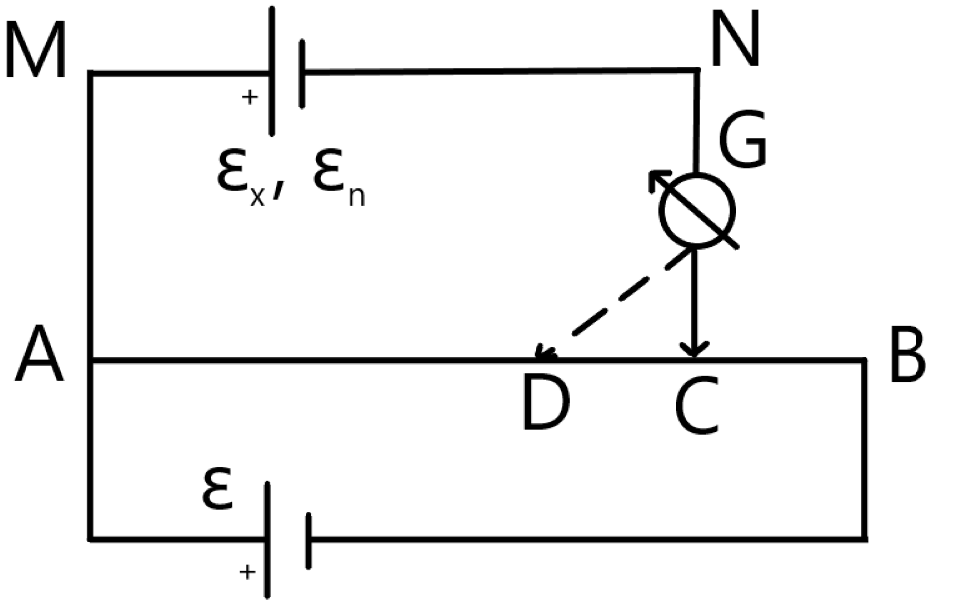
\includegraphics[scale=0.3]{scheme-1}
	\end{center}
	\caption{Компенсационная схема}
\end{figure}

Здесь: $\mathcal{E}$ - источник питания $\mathcal{E}_x$ - исследуемый элемент $\mathcal{E}_n$ - нормальный (контрольный) элемент, $G$ - гальванометр.  

Если подключить вольтметр напрямую к источнику ЭДС, то полное сопротивление будет состоять не только из сопротивления вольтметра, но и из сопротивления источника:
$$R = R_V + r,$$
где $R_V$ - сопротивление вольтметра, $r$ - сопротивление источника ЭДС.

Из \eqref{Om} следует:
\begin{equation}
	\mathcal{E} = IR_V + Ir
\end{equation}

Слагаемое $IR_V$ представляет собой напряжение, которое показывает вольтметр, и это показание отличается от ЭДС на величину падения напряжения на внутреннем сопротивлении источника.

И если подключить $\mathcal{E}$ и  $\mathcal{E}_x$ параллельно, и $\mathcal{E} > \mathcal{E}_x$, то на реохорде $AB$ мы сможем найти точку $C$, при которой ток на $AMNC$ будет равен нулю. 
Применив второй закон Кирхгофа для контура $AMNCA$, имеем:
\begin{equation}\label{Kirchhoff}
	I_2R_{AMNC} - I_1R_{AC} = -\mathcal{E}_x
\end{equation}
И так как $I_2 = 0$:
\begin{equation}\label{I1_1}
	I_1R_{AC} = \mathcal{E}
\end{equation}
Таким образом, падение напряжения на $AC$, создаваемое $\mathcal{E}$ компенсирует ЭДС исследуемого нами элемента.

Затем мы меняем $\mathcal{E}_x$ на $\mathcal{E}_n$ (нормальный источник). Передвигая $C$ мы добиваемся $I_2 = 0$ и в этом случае падение напряжение на $AD$ компенсирует ЭДС нормального элемента;
\begin{equation}\label{I1_2}
	I_1R_{AD} = \mathcal{E}
\end{equation}

Также нужно учесть, что $I_1$ в \eqref{I1_1} и \eqref{I1_2} не меняется, так как данный ток идёт по контуру $AB$, который, вообще говоря, не меняется. Откуда мы получаем:
\begin{equation}\label{close_final}
	\mathcal{E}_x = \mathcal{E}_n\frac{R_{AC}}{R_{AD}} 
\end{equation}
Так как сопротивление на любом участке реохорда равно:
$$ R = \rho \frac{l}{S},$$
где $l$ - длина проводника, $S$ - площадь поперечное сечение, $\rho$ - удельное электрическое сопротивление (зависящее от свойств материала).
В нашем случае $\rho, S = const$, при подставлении в \eqref{close_final} данные константы сократятся, и мы получим:
\begin{equation}
	\mathcal{E}_x = \mathcal{E}_n\frac{l_{AC}}{l_{AD}},
\end{equation}
где $l_{AC}$ и $l_{AD}$ - длины участков реохорда $AC$ и $AD$ соответственно.

\newpage

\section{План работы}
\begin{enumerate}
\item Собрать схему как на рисунке. Кнопочный ключ $K_1$ используется для предохранения схемы от экстратоков замыкания.
\item Магазины сопротивлений $M.C.$ поставить на максимум.
\item Двойным ключом $К_2$ подсоединить неизвестный элемент $\mathcal{E}_x$ 
\item Замнуть ключ $K_1$ и, двигая рычаг реохорда, выставить точку $C$, при которой ток $I_2$ на гальванометре $G$ будет равен нулю. 
\item Уменьшая сопротивление $M.C.$ ожидать окончательной компенсации тока.
\item Снять значение $l_x$ соответствующее длине участка $AC$ при полной компенсации.
\item Вернуть $M.C.$ в максимальное значение.
\item Переключить ключ $К_2$ на нормальный элемент. Повторить пункты (4, 5) Снять значение $l_n$.
\item Провести вышеуказанные пункты несколько раз для выявления случайной погрешности.
\item Внести полученные данные в таблицу.
\end{enumerate} 



\newpage
\section{Ход работы}









\end{document}



